% Template for PLoS
% Version 3.5 March 2018
%
% % % % % % % % % % % % % % % % % % % % % %
%
% -- IMPORTANT NOTE
%
% This template contains comments intended 
% to minimize problems and delays during our production 
% process. Please follow the template instructions
% whenever possible.
%
% % % % % % % % % % % % % % % % % % % % % % % 
%
% Once your paper is accepted for publication, 
% PLEASE REMOVE ALL TRACKED CHANGES in this file 
% and leave only the final text of your manuscript. 
% PLOS recommends the use of latexdiff to track changes during review, as this will help to maintain a clean tex file.
% Visit https://www.ctan.org/pkg/latexdiff?lang=en for info or contact us at latex@plos.org.
%
%
% There are no restrictions on package use within the LaTeX files except that 
% no packages listed in the template may be deleted.
%
% Please do not include colors or graphics in the text.
%
% The manuscript LaTeX source should be contained within a single file (do not use \input, \externaldocument, or similar commands).
%
% % % % % % % % % % % % % % % % % % % % % % %
%
% -- FIGURES AND TABLES
%
% Please include tables/figure captions directly after the paragraph where they are first cited in the text.
%
% DO NOT INCLUDE GRAPHICS IN YOUR MANUSCRIPT
% - Figures should be uploaded separately from your manuscript file. 
% - Figures generated using LaTeX should be extracted and removed from the PDF before submission. 
% - Figures containing multiple panels/subfigures must be combined into one image file before submission.
% For figure citations, please use "Fig" instead of "Figure".
% See http://journals.plos.org/plosone/s/figures for PLOS figure guidelines.
%
% Tables should be cell-based and may not contain:
% - spacing/line breaks within cells to alter layout or alignment
% - do not nest tabular environments (no tabular environments within tabular environments)
% - no graphics or colored text (cell background color/shading OK)
% See http://journals.plos.org/plosone/s/tables for table guidelines.
%
% For tables that exceed the width of the text column, use the adjustwidth environment as illustrated in the example table in text below.
%
% % % % % % % % % % % % % % % % % % % % % % % %
%
% -- EQUATIONS, MATH SYMBOLS, SUBSCRIPTS, AND SUPERSCRIPTS
%
% IMPORTANT
% Below are a few tips to help format your equations and other special characters according to our specifications. For more tips to help reduce the possibility of formatting errors during conversion, please see our LaTeX guidelines at http://journals.plos.org/plosone/s/latex
%
% For inline equations, please be sure to include all portions of an equation in the math environment.  For example, x$^2$ is incorrect; this should be formatted as $x^2$ (or $\mathrm{x}^2$ if the romanized font is desired).
%
% Do not include text that is not math in the math environment. For example, CO2 should be written as CO\textsubscript{2} instead of CO$_2$.
%
% Please add line breaks to long display equations when possible in order to fit size of the column. 
%
% For inline equations, please do not include punctuation (commas, etc) within the math environment unless this is part of the equation.
%
% When adding superscript or subscripts outside of brackets/braces, please group using {}.  For example, change "[U(D,E,\gamma)]^2" to "{[U(D,E,\gamma)]}^2". 
%
% Do not use \cal for caligraphic font.  Instead, use \mathcal{}
%
% % % % % % % % % % % % % % % % % % % % % % % % 
%
% Please contact latex@plos.org with any questions.
%
% % % % % % % % % % % % % % % % % % % % % % % %

\documentclass[10pt,letterpaper]{article}
\usepackage[top=0.85in,left=2.75in,footskip=0.75in]{geometry}

% amsmath and amssymb packages, useful for mathematical formulas and symbols
\usepackage{amsmath,amssymb}

% Use adjustwidth environment to exceed column width (see example table in text)
\usepackage{changepage}

% Use Unicode characters when possible
\usepackage[utf8x]{inputenc}

% textcomp package and marvosym package for additional characters
\usepackage{textcomp,marvosym}

% cite package, to clean up citations in the main text. Do not remove.
\usepackage{cite}

% Use nameref to cite supporting information files (see Supporting Information section for more info)
\usepackage{nameref,hyperref}

% line numbers
\usepackage[right]{lineno}

% ligatures disabled
\usepackage{microtype}
\DisableLigatures[f]{encoding = *, family = * }

% color can be used to apply background shading to table cells only
\usepackage[table]{xcolor}

% array package and thick rules for tables
\usepackage{array}

% create "+" rule type for thick vertical lines
\newcolumntype{+}{!{\vrule width 2pt}}

% create \thickcline for thick horizontal lines of variable length
\newlength\savedwidth
\newcommand\thickcline[1]{%
  \noalign{\global\savedwidth\arrayrulewidth\global\arrayrulewidth 2pt}%
  \cline{#1}%
  \noalign{\vskip\arrayrulewidth}%
  \noalign{\global\arrayrulewidth\savedwidth}%
}

% \thickhline command for thick horizontal lines that span the table
\newcommand\thickhline{\noalign{\global\savedwidth\arrayrulewidth\global\arrayrulewidth 2pt}%
\hline
\noalign{\global\arrayrulewidth\savedwidth}}


% Remove comment for double spacing
%\usepackage{setspace} 
%\doublespacing

% Text layout
\raggedright
\setlength{\parindent}{0.5cm}
\textwidth 5.25in 
\textheight 8.75in

% Bold the 'Figure #' in the caption and separate it from the title/caption with a period
% Captions will be left justified
\usepackage[aboveskip=1pt,labelfont=bf,labelsep=period,justification=raggedright,singlelinecheck=off]{caption}
\renewcommand{\figurename}{Fig}

% Use the PLoS provided BiBTeX style
\bibliographystyle{plos2015}
% Remove brackets from numbering in List of References
\makeatletter
\renewcommand{\@biblabel}[1]{\quad#1.}
\makeatother



% Header and Footer with logo
\usepackage{lastpage,fancyhdr,graphicx}
\usepackage{epstopdf}
%\pagestyle{myheadings}
\pagestyle{fancy}
\fancyhf{}
%\setlength{\headheight}{27.023pt}
%\lhead{\includegraphics[width=2.0in]{PLOS-submission.eps}}
\rfoot{\thepage/\pageref{LastPage}}
\renewcommand{\headrulewidth}{0pt}
\renewcommand{\footrule}{\hrule height 2pt \vspace{2mm}}
\fancyheadoffset[L]{2.25in}
\fancyfootoffset[L]{2.25in}
\lfoot{\today}

%% TEMPORARY FIGURES (REMOVE BEFORE SUBMISSION)
% \usepackage[svgpath=./figs/]{svg}
\usepackage{graphicx}
\graphicspath{{./betaSeriesSimulations/outputs/}{./BetaSeriesRealDataAnalysis/nibsAnalysis/outputs/}{./BetaSeriesRealDataAnalysis/firstLevelAnalysis/outputs/}{./BetaSeriesRealDataAnalysis/introductionFigures/outputs/}}
\usepackage{float}
\usepackage[caption=false]{subfig}
\usepackage{csvsimple}
\usepackage{chngcntr}
\counterwithout{figure}{section}

%% Include all macros below

\newcommand{\lorem}{{\bf LOREM}}
\newcommand{\ipsum}{{\bf IPSUM}}

%% END MACROS SECTION


\begin{document}
\vspace*{0.2in}

% Title must be 250 characters or less.
\begin{flushleft}
{\Large
\textbf\newline{Beta series correlations} % Please use "sentence case" for title and headings (capitalize only the first word in a title (or heading), the first word in a subtitle (or subheading), and any proper nouns).
}
\newline
% Insert author names, affiliations and corresponding author email (do not include titles, positions, or degrees).
\\
James Kent\textsuperscript{1*},
Chandramallika Basak\textsuperscript{2}
Michelle Voss\textsuperscript{1},
%Name3 Surname\textsuperscript{2,3\textcurrency},
%Name4 Surname\textsuperscript{2},
%Name5 Surname\textsuperscript{2\ddag},
%Name6 Surname\textsuperscript{2\ddag},
%Name7 Surname\textsuperscript{1,2,3*},
%with the Lorem Ipsum Consortium\textsuperscript{\textpilcrow}
\\
\bigskip
\textbf{1} Psychology Department, University of Iowa, Iowa City, Iowa, United States
\textbf{2} School of Behavioral and Brain Science, University of Texas at Dallas, Dallas, Texas, United States
%\\
%\textbf{2} Affiliation Dept/Program/Center, Institution Name, City, State, Country
%\\
%\textbf{3} Affiliation Dept/Program/Center, Institution Name, City, State, Country
%\\
\bigskip

% Insert additional author notes using the symbols described below. Insert symbol callouts after author names as necessary.
% 
% Remove or comment out the author notes below if they aren't used.
%
% Primary Equal Contribution Note
%\Yinyang These authors contributed equally to this work.

% Additional Equal Contribution Note
% Also use this double-dagger symbol for special authorship notes, such as senior authorship.
%\ddag These authors also contributed equally to this work.

% Current address notes
% \textcurrency Current Address: Dept/Program/Center, Institution Name, City, State, Country % change symbol to "\textcurrency a" if more than one current address note
% \textcurrency b Insert second current address 
% \textcurrency c Insert third current address

% Deceased author note
% \dag Deceased

% Group/Consortium Author Note
% \textpilcrow Membership list can be found in the Acknowledgments section.

% Use the asterisk to denote corresponding authorship and provide email address in note below.
* james-kent@uiowa.edu

\end{flushleft}
% Please keep the abstract below 300 words
\section*{Abstract}
Cognitive tasks drive discovery in cognitive neuroscience by connecting behavior and representation
of the behavior in the brain.
Taking a network perspective is undeniably important to identify the representations.
Beta series correlations are an increasingly popular measure to estimate which brain regions correlate with
each other during different event conditions within an MRI scanner.
The region to region correlations serve as a marker for the brain network representation
for the event condition.
Two common ways to generate beta series are Least Squares All (LSA) and
Least Squares Separate (LSS).
However, LSS and LSA have not been systematically compared with simulations and real data
to identify which method is more sensitive to detect region to region correlation differences
between event conditions.
We compared LSA and LSS by simulating responses across a variety of
experimental designs and testing LSS and LSA performance on a real dataset.
Our simulations show LSS outperforms LSA across a variety of inter-event
intervals and numbers of total events.
In contrast, real data does not show an advantage of one method over the other.
This research shows the importance of validation using both simulations
and real data and impacts how future studies should design their tasks
to improve detectability of conditional organization of brain networks.

\linenumbers

% Use "Eq" instead of "Equation" for equation citations.
\section*{Introduction}
\label{intro}

The field of human neuroimaging has moved towards interrogating networks of brain regions.
Broadly defined, a brain network is a collection of brain regions who share information ~\cite{Uddin2019}.
Brain networks have primarily been investigated while at rest, but there
is rising popularity to observe brain networks while participants perform tasks ~\cite{Cole2014a}.
There is also rising popularity to measure dynamic features of brain networks over time ~\cite{Sakoglu2008,Hindriks2016}.
However, There has not been significant validation and investigation of brain networks
when participants engage in tasks with interleaved conditions that could induce
different brain networks dynamically ~\cite{Di2019a}.
In other words measuring brain networks have not been validated within fast event-related designs ~\cite{Buckner1998}.
We seek to validate and compare two methods that can measure brain responses to events that occur
close in time.

The overarching method being investigated is beta series correlations (BSC) ~\cite{Rissman2004,Mumford2012,Turner2012a,Abdulrahman2016}
There are two main approaches to estimate the Beta Series for BSC: Least Squares All (LSA) and Least Squares Separate (LSS) ~\cite{Mumford2012}.
Both approaches of beta series estimation seek to derive single event estimates that represent a brain region's
(or voxel's) activity at each individual event.
An event is defined as "a stimulus or participant response recorded during a task." ~\cite{Gorgolewski2016}
Where task is defined as "a set of structured activities performed by the participant." ~\cite{Gorgolewski2016}
The single event estimates become difficult to estimate when events are close together,
in other words, less than the time it takes for the Blood Oxygen Level Dependent (BOLD) response to return to baseline.
Such designs are called fast event related designs which are commonly used in cognitive neuroscience \ref{fig:introhrf}.

\begin{figure}[H]
  \centering
  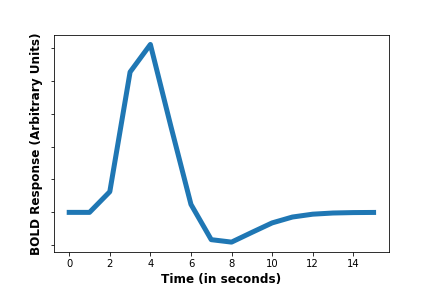
\includegraphics[width=\textwidth]{introduction-hrf}
  \caption{
    Model of the Hemodynamic Response Function (HRF) ~\cite{Glover1999} at a
    typical resolution of an fMRI scan (2 seconds).
    The x-axis represents time in seconds and the y-axis is arbitrary units.
    Fast event related designs with inter event intervals (IEIs) at or faster than time to peak
    response (e.g., 4-6 seconds), need to account for the overlapping signals.
  }
  \label{fig:introhrf}
\end{figure}

The BOLD response is an indirect measure of neuronal activity that take approximately 6 seconds to
peak and around 16-32 seconds to effectively resolve ~\cite{Glover1999}.
If events are occurring (on average) 4 seconds apart, the difficulty of single event estimation
becomes apparent.
One does not know whether BOLD activity should be attributed to a target event or an
adjacent event.
LSA and LSS approach this problem differently.
LSA, namely, ignores this problem by calculating a high variance, but low bias measure;
while LSS calculates a lower variance; but more biased measure.
To understand how LSA and LSS approach single event estimation, it is necessary to introduce
the General Linear Model (GLM).
GLMs are a mainstay in the neuroimaging literature, allowing researchers to model
a curve that approximates the BOLD response shape and linearly scale the curve
to best match the data ~\cite{Friston1995}.
The multiplicative that linearly scales the model BOLD response is known as a beta.
The beta in the GLM is where the "beta" in beta series comes from.
This beta is often interpreted as the amplitude of the response, which is true when the
model approximates the shape of the BOLD response well, and becomes less clear when
the model does not.
In a traditional GLM, events of the same type will be grouped together
to provide a robust estimate of whether a particular region or set of regions are
active relative to some baseline or another condition ~\ref{fig:introGLM}.

\begin{figure}[H]
  \centering
  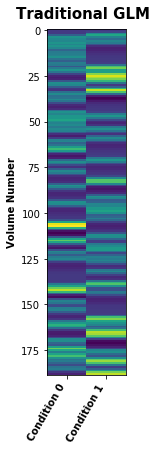
\includegraphics{introduction-normalGLM}
  \caption{
    An example of a design matrix seen in a traditional GLM used in fMRI ~\cite{Friston1995}.
    There is a single column for each condition, resulting in two columns (intercept column ignored for clarity).
    With this design you can answer questions about which voxels are more or less active in one condition
    versus another, but you cannot see which voxels vary together over stimulus presentations.
  }
  \label{fig:introGLM}
\end{figure}

Grouping together events of the same type, however, does not tell you which regions are acting in concert
in response to the event type.
The traditional GLM outputs a single beta estimate per event type, to measure which which regions
are acting in concert; you would need a beta estimate per event.
It could be the case that for half of the events of the same type two regions are active,
and for the other half, another two regions are active.
The traditional GLM will not be able differentiate the different pairs of regions.
LSS and LSA, on the other hand, propose to be able to separate the different pairs of regions.
LSA takes a variant of the traditional GLM whereby instead of providing a beta
estimate for a group of events, each event gets its own beta estimate in a single GLM ~\ref{fig:introlsa}.

\begin{figure}[H]
  \centering
  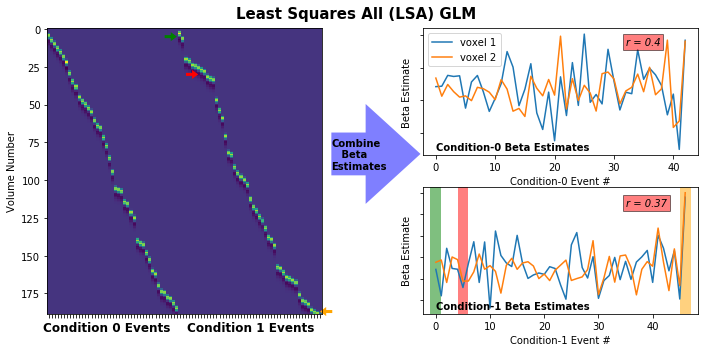
\includegraphics[width=\textwidth]{introduction-lsa}
  \caption{
    Left shows an example design matrix for LSA where each event gets its own column.
    Since we receive a beta estimate per column, we end up with as many beta estimates as there
    are events.
    We can combine those beta estimates to create a beta series (Right) for each condition.
    In this example we measured beta series for two voxels, allowing us to
    correlate the betaseries from one voxel to another.
    We can perform the correlation for the two conditions.
    The arrows on the design matrix (left) correspond to the beta estimates of those events
    on the shaded regions (right).
  }
  \label{fig:introlsa}
\end{figure}

LSS differs from LSA by fitting a separate GLM for each event, where in each model a target
event is fit and the rest of the events are grouped together and given separate beta estimates ~\ref{fig:introlss}.
Placing all other events into a single regressor is how LSS was introduced, but as shown in \ref{fig:introlss},
each event type has its own regressor, which is referred to as LSS-N in other papers.
We will refer to LSS-N as LSS for the remainder of the manuscript.

\begin{figure}[H]
  \centering
  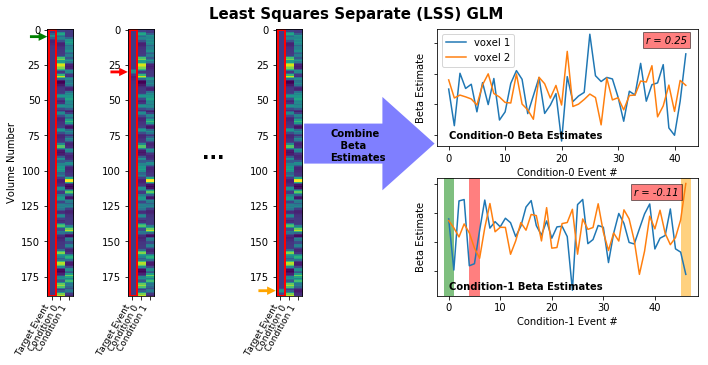
\includegraphics[width=\textwidth]{introduction-lss}
  \caption{
    Left shows an example design matrix for LSS where each event gets its own model
    (intercept excluded for clarity).
    The target event (outlined in red) comes from either condition 0 or 1.
    For example, if the target event is from condition 1, the remaining condition 1 events
    get their own column, and all of the condition 0 events get their own column
    Since we receive a beta estimate per model, we end up with as many beta estimates as there
    are events.
    We can combine those beta estimates to create a beta series (Right) for each condition.
    In this example we measured beta series for two voxels, allowing us to
    correlate the betaseries from one voxel to another.
    We can perform the correlation for the two conditions.
    The arrows on the design matrix (left) correspond to the beta estimates of those events
    on the shaded regions (right).
  }
  \label{fig:introlss}
\end{figure}

The target event estimate for each model is taken to form a beta series.
Harkening back to the sluggish BOLD response, LSA suffers when the events are close together,
since the GLM cannot reliably attribute which BOLD response should correspond to which event ~\ref{fig:introGLM}.
LSS attempts to reduce the model confusion by only having one single event estimate per model,
so the non-target events have their beta influenced by multiple observations, loosening the
constraint that adjacent events to the target event need to be orthogonal (i.e., independent) of each other.
While previous work has simulated beta series and evaluated beta series on real data,
several key gaps remain ~\cite{Mumford2014a,Mumford2012,Turner2012a,Abdulrahman2016,Cisler2012,Arco2018}.
One, simulations have not taken into account realistic noise structure of fMRI data such as autocorrelations, movement, and phsyiological noise.
Two, simulations have not used optimized fast event related designs, only randomly selected designs. 
Three, empirical selections of signal to noise ratios have not been considered,
ratios were chosen without justification in previous work.
Four, a quantitative comparison/validation of LSA and LSS condition contrasts for BSC has not been done.
The present work fills these gaps and provides recommendations for further research
using LSA and LSS.
Important terms used used throughout the paper are presented \ref{table0}.

\begin{table}[H]
  \begin{adjustwidth}{0in}{0in} % Comment out/remove adjustwidth environment if table fits in text column.
  \centering
  \caption{
  {\bf Acronym Definitions}}
  \begin{tabular}{|l|l|p{60mm}|}
  \hline
  Name & Acronym & Definition\\ \thickhline
  Least Squares All & $LSA$ & beta estimation method where each event gets a regressor in the same model\\ \hline
  Least Squares Separate & $LSS$ & beta estimation method where each event gets a separate model\\ \hline
  Contrast Noise Ratio & $CNR$ & $A_S/\sigma_N$, amplitude of signal ($A_S$) divided by standard deviation of the noise ($\sigma_N$)\\ \hline
  Activation Variation Noise Ratio & $AVNR$ & $\sigma_S/\sigma_N$, standard deviation of signal ($\sigma_S$) divided by standard deviation of the noise ($\sigma_N$)\\ \hline
  \end{tabular}

  Definitions of the main acronyms use in this paper.
  $CNR$ and $AVNR$ definitions are found in Welvaert (2013)~\cite{Welvaert2013a}.
  \label{table0}
  \end{adjustwidth}
  \end{table}

\section*{Materials and methods}
\label{methods}

Testing and validation of beta series correlations followed three stages.
First, beta series correlations were tested in simulations across different
optimized experimental designs.
Second, beta series correlations were tested in simulations using an experimental
design that was used to collect real data.
Third, beta series correlations were validated in real task data collected from
participants.
Resting state data collected from the same participants was used as a null
control for beta series correlations.
Since there is no expectation of betaseries correlations to change
during resting state, we can get a measure of expected spurious results found
in beta series correlations.

\subsection*{BetaSeries Correlations}
\label{methods:bsc}

\subsubsection*{Beta Series Modeling}
\label{methods:bsc_model}

The LSS models were generated for each event in
the task following the method described in \cite{Turner2012a}, using
Nistats 0.0.1b2.\\
Prior to modeling, preprocessed data were masked, and mean-scaled over
time.
Mean scaling was not applied when calculating CNR and AVNR so the
beta estimates would be in the original BOLD units.
For each event, preprocessed data were subjected to a GLM
in which the event was modeled with its own regressor, while
all other events from that condition were modeled in a second regressor,
and other conditions were modeled in their own regressors.
So if the task has the conditions switch, repeat, and single, 
a single GLM would have 4 event regressors, 1 for the target
event, and 3 for the remaining conditions.

The LSA model was generated following the method described in
\cite[Rissman (2004)]{Rissman2004}, using Nistats 0.0.1b2.
Each event was given its own regressor in a single GLM, such that
if the experiment had 100 events, there would be 100 regressors in the GLM.

Each event regressor was convolved with a glover hemodynamic response
function\cite{Glover1999}.
In addition to event regressors, average white matter signal, average csf signal,
cosine basis set high pass regressors, the initial four non stead state volumes, 
and motion outliers were included
in the model as calculated in the Preparing fMRI section.
AR(1) prewhitening was applied in each model to account
for temporal autocorrelation.

After fitting each model, the parameter estimate (i.e., beta) map
associated with the target event's regressor was retained and
concatenated into a 4D image with all other events from the same
condition, resulting in a set of $X$ 4D images where $X$ refers to the
number of conditions in the task.
The number of volumes in each 4D image represents the number of events in that condition.


\subsubsection*{Atlas Correlation Analysis}
\label{methods:atlas-corr-analysis}

The beta series 4D image for each condition in the task was subjected to
an region of interest to region of interest (ROI-to-ROI) correlation analysis
to produce condition-specific correlation matrices.
For the simulation data, ROI-to-ROI correlations were calculated by
treating each voxel as an ROI.
In the real data; two atlases were used to generate ROI-to-ROI correlation matrices.
We created an activation atlas representing regions that were
consistently activated across event conditions (see \nameref{methods:task-switch}).
This atlas has coverage across several cortical and subcortical regions.
The second atlas, Schaefer Atlas (400 parcels, 17 networks)\cite{Schaefer2017}, was
used to comprehensively cover the cortex and demonstrate robustness of results.

Outlier beta estimate volumes were identified and discarded using a
modified Nipype function for outlier detection
(\href{https://github.com/HBClab/NiBetaSeries/blob/a45c0a1f/src/nibetaseries/interfaces/nilearn.py#L153}{see here}) ~\cite{Crosby1994}.
The correlation coefficient estimator used for generating correlation matrices
was empirical covariance, as implemented in Nilearn 0.4.2
\cite{Abraham2014}.
Correlation coefficients were converted to normally-distributed z-values using
Fisher's r-to-z conversion \cite{Fisher1915}.

In the participant data, BSC generated correlation matrices for each condition (switch, repeat, single),
each method, (LSA and LSS), each data type (real and null), and each participant (N=40).
The first check performed was contrasting the real switch condition and null switch condition
to ensure BSC from a task are different than BSC from null data.
A paired ttest was run on each ROI-ROI pair for the activation atlas, totaling 210 comparisons
between task and null.
We next contrasted $switch - single$, $repeat - single$, and $switch - repeat$, for LSS/LSA in both
real and null data.

Since we do not have a ground truth for which ROI-ROI pairs should be different between conditions,
we used permutation tests on the correlation matrices to ascertain whether we observed a greater number
of statistically significant ROI-ROI pairs than would be expected.
We did not use false discovery rate correction on the observed p-values since we were not interested in
which specific ROI-ROI pair correlations were likely to be true positives, but rather if the number of positives
observed would be expected by chance alone or if LSS/LSA likely detected an overall difference between event conditions
We shuffled each ROI-ROI pair within each participant such that any ROI-ROI correlation would remain
in their own condition, or be swapped.
We shuffled every participants' ROI-ROI pairs for 1000 iterations and ran a paired ttest on every ROI-ROI pair
for each iteration.
We then summed the total number of statistically significant ROI-ROI pairs for each iteration and used
to form the distribution of expected results.
For example, if we observed 10 significant ROI-ROI pairs in our real data, we could permute the data
with 5 iterations resulting in $[5, 3, 12, 7, 10]$.
To determine our p-value, we would count the number of permuted results that at least as large as
our observed number and divide that number by the total number of iterations.
In this example, 2 values are at least as large as our observed result (10 and 12), so our
p-value would be $2/5$ or 0.4.
Since we are using 1000 iterations, our p-values will provide a more exact estimates than the example.
(\href{https://github.com/jdkent/BetaSeriesRealDataAnalysis/blob/90fafb5b83b2e1bfade61a9fb1a87f225efaa95f/nibsAnalysis/BetaSeriesAnalysis.ipynb}{see here for relevant code})

\subsection*{Beta Series Correlation Simulations}
\label{methods:bsc-simulations}

To assess the validity and power of beta series correlations,
we simulated two voxels of fMRI timeseries data and convolved short (0.2 second)
task onsets with double gamma functions
and added the responses to the timeseries~\cite{Glover1999,Welvaert2011}.
We used fmrisim from the brainiak toolbox\cite{Ellis2020} to generate a
two voxel fMRI timeseries containing drift, autocorrelation ($\rho$ = 0.5), phsysiological noise,
task related movement, and scanner noise \ref{fig:simulation_example}.
Noise features were all weighted equally in the simulations.

\begin{figure}[H]
  \centering
  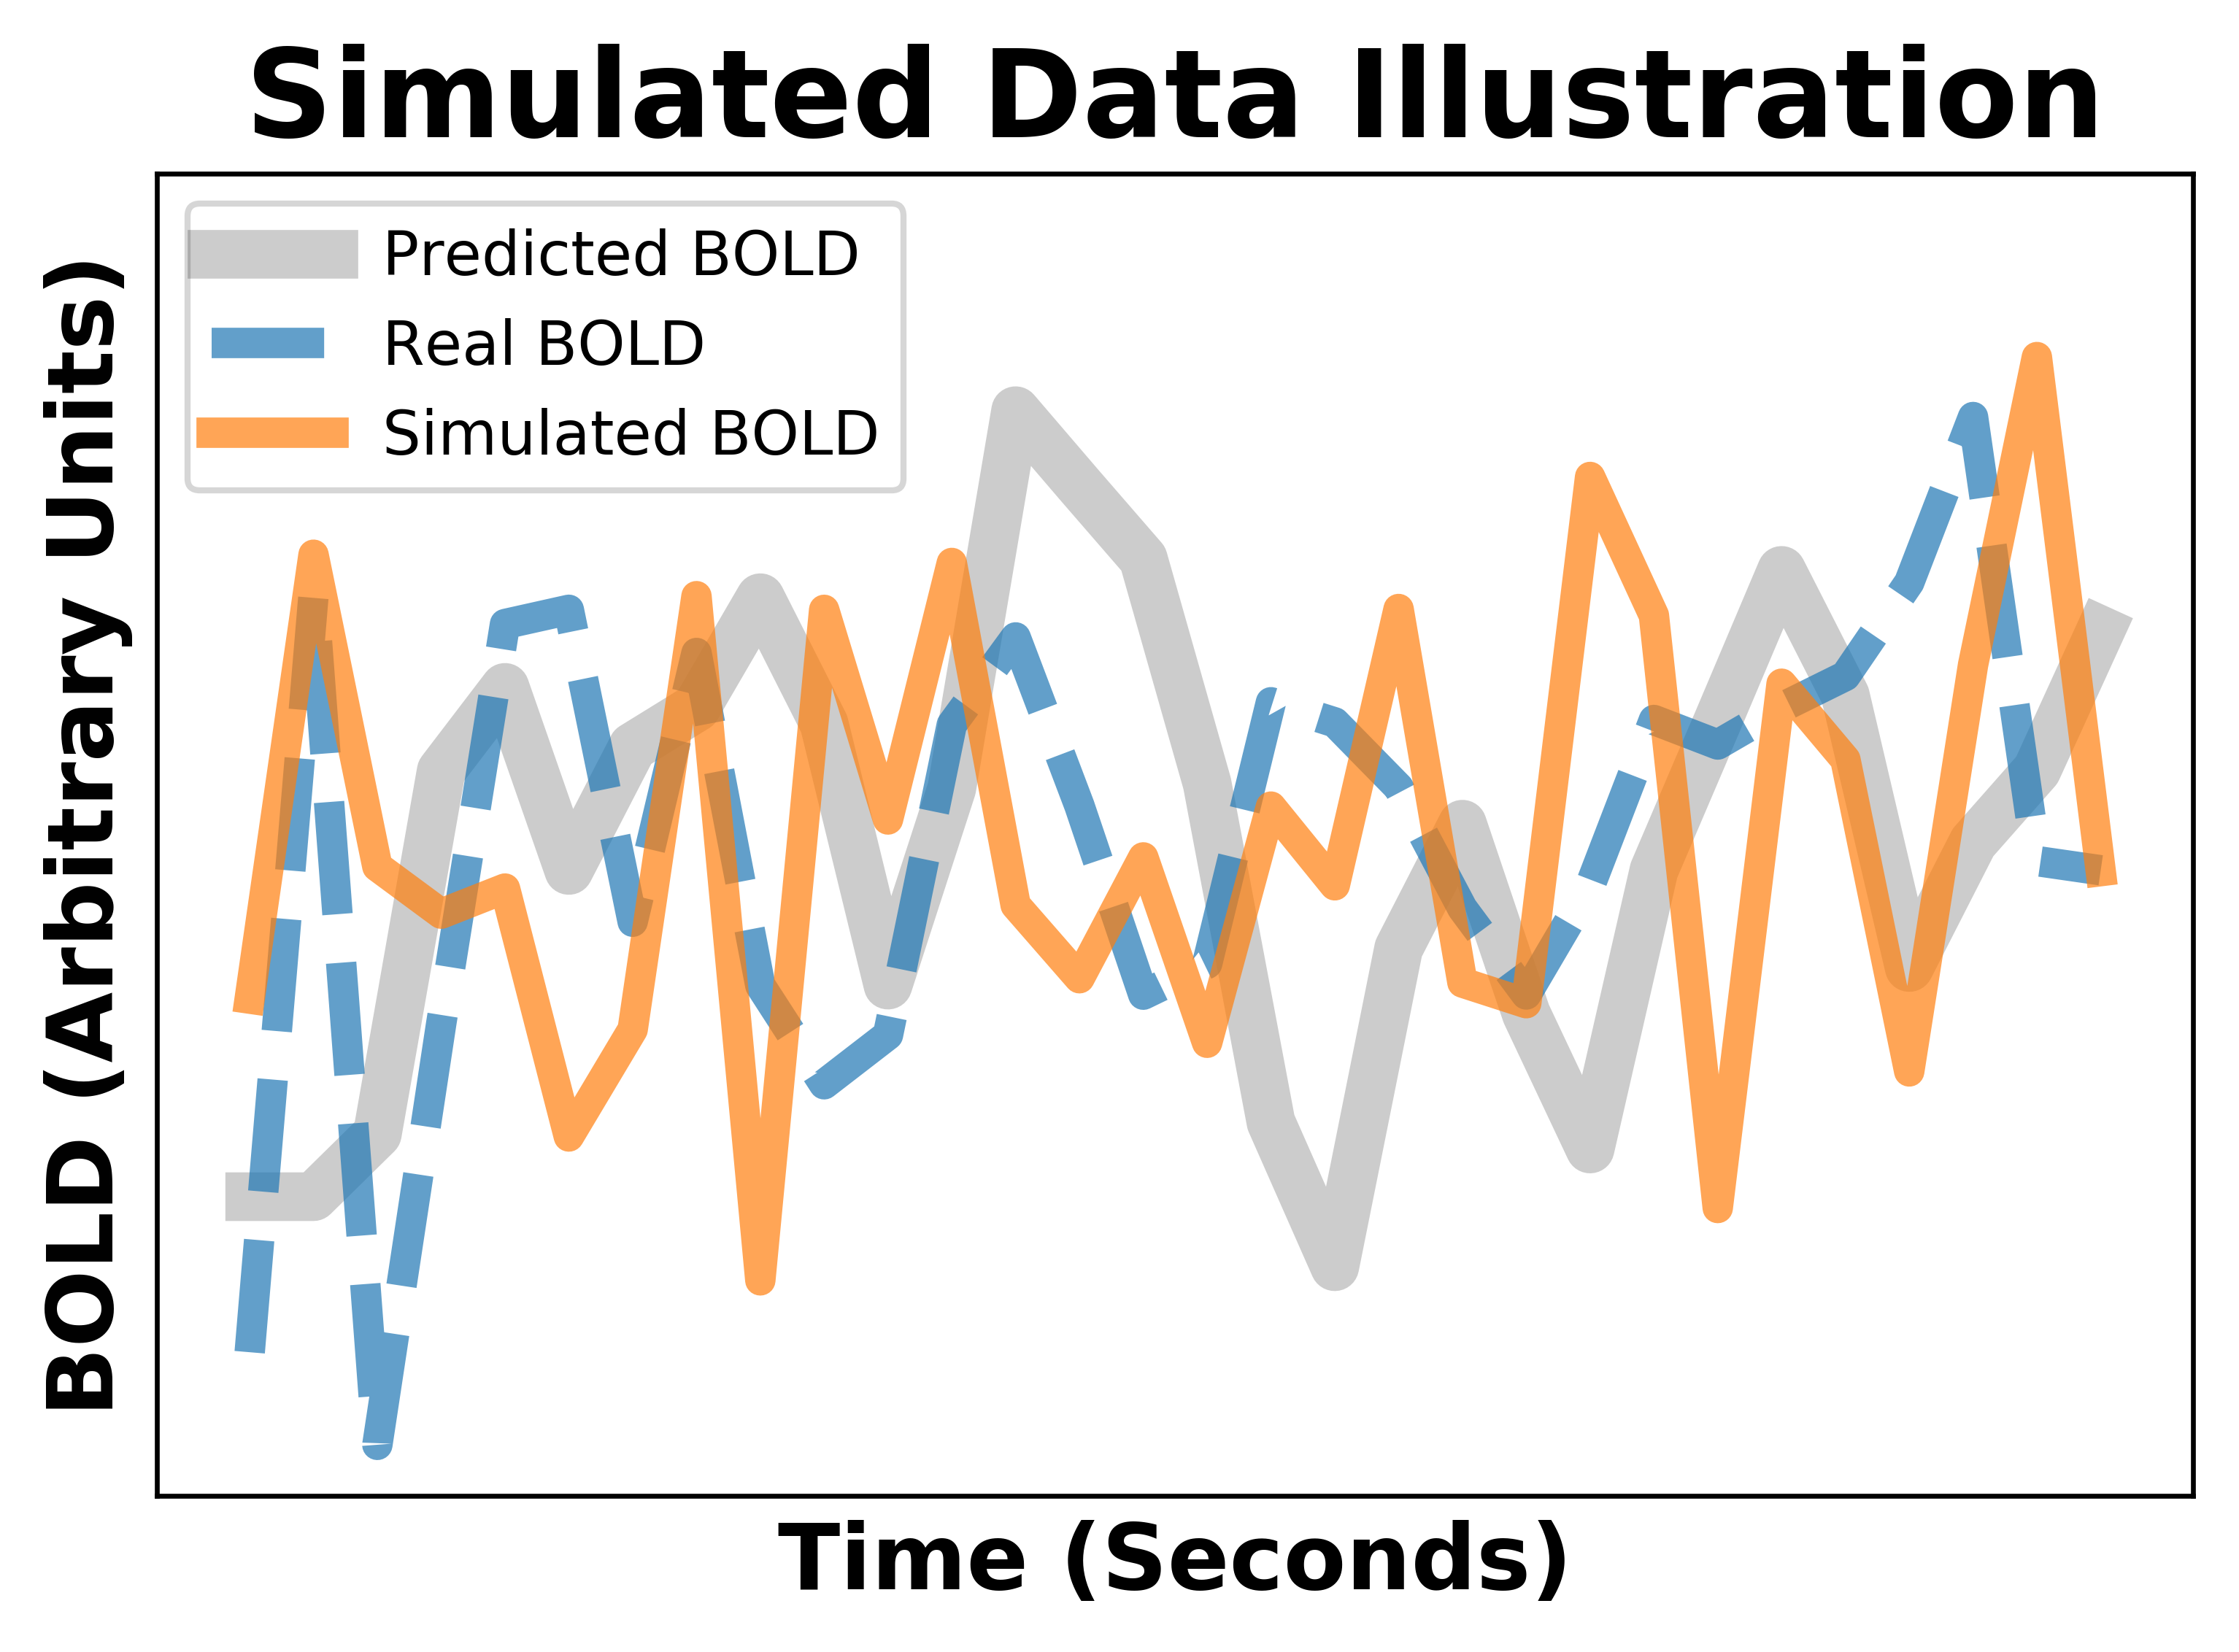
\includegraphics{methods-simulation_example}
  \caption{
    Example of predicted BOLD from a task design (thick grey line), real BOLD
    from a participant (see \nameref{methods:task-switch}), and simulated BOLD
    from fmrisim\cite{Ellis2020}.
  }
  \label{fig:simulation_example}
\end{figure}

For all simulations the time of repetition was set at 2 seconds.
We varied the contrast-to-noise ratio (CNR) using the amplitude of the activation
divided by the standard deviation of the noise~\cite{Welvaert2013a}.
In other words, we used the average of the beta estimates and divided by the standard
deviation of the residuals output by the LSA model.
Another parameter deemed critical by previous work is the standard deviation
of the raw beta estimates relative to the standard deviation of the noise~\cite{Abdulrahman2016},
so we varied that measure as well.
Since Abdulrahman \& Henson (2016)\cite{Abdulrahman2016} also called their measure
CNR, we've decided to rename it as Activation Variance to Noise Ratio (AVNR), to
contrast it with our definition of CNR.

To generate realistic numbers for simulating timeseries at varying CNRs and AVNRs
we used an unpublished dataset on task switching in older adults (N=40).
We ran LSS/LSA to get both event estimates of activation (i.e., betas)
as well as residuals from the model.
To calculate CNR, several steps were taken.
First, we masked the betaseries using the Schaefer or Activation atlases (see \nameref{methods:atlas-corr-analysis}).
Second, we took the absolute value of all masked beta estimates for a participant.
Third, we took the median beta estimates over all event volumes resulting
in a median beta estimate amplitude for all ROIs.
Fourth, we took the standard deviation of the residuals for each ROI.
Fifth, we divided the median amplitude beta estimates by the standard deviation of the residuals
for each ROI.
Sixth, we took either the mean or max CNR across all ROIs to provide a reasonable estimate
and upper bound of CNR.
Calculating AVNR followed the same procedure as CNR with the exception of the first two steps.
First, we took the standard deviation of the beta estimates, then we followed steps three through six above
on the standard deviation of the beta estimates (as opposed the amplitude).
(\href{https://github.com/jdkent/BetaSeriesRealDataAnalysis/blob/90fafb5b83b2e1bfade61a9fb1a87f225efaa95f/nibsAnalysis/cnr_trial_variability.ipynb}{see here for the relevant code})

\begin{table}[H]
\begin{adjustwidth}{0in}{0in} % Comment out/remove adjustwidth environment if table fits in text column.
\centering
\caption{
{\bf Summary of AVNR and CNR measures in Real Data}}
\begin{tabular}{|l+l+l|l|l|l|}
\hline
Atlas & Method & CNR (mean) & CNR (max) & AVNR (mean) & AVNR (max)\\ \thickhline
$Schaefer$ & $LSS$ & 0.71 & 1.81 & 1.03 & 2.33\\ \hline
$Activation$ & $LSS$ & 0.99 & 1.58 & 1.42 & 2.18\\ \hline
$Schaefer$ & $LSA$ & 1.02 & 2.48 & 1.54 & 3.61\\ \hline
$Activation$ & $LSA$ & 1.42 & 2.18 & 2.15 & 3.26\\ \hline
\end{tabular}
The average and maximum CNR and AVNR for both atlases (Schaefer and Activation)
as well as estimation method (LSS and LSA).
LSS tends to give lower CNR/AVNR since the measure sacrifices
variance for bias, unlike LSA, which remains unbiased.
\label{table1}
\end{adjustwidth}
\end{table}

We derived CNRs of 1 and 2 as and AVNRs of 1 and 2 as reasonable values from the dataset \ref{table1}.
We can manipulate CNR and AVNR independently to determine whether simulated BOLD response variation
impact beta series correlation's ability to recapture the true correlation or if the simulated BOLD
response magnitude is more important.
The choice of onset times was varied based on average inter-event-interval (IEIs).
The IEI is the time from the previous event onset to the next event onset.
We chose average IEIs at 2, 4, 6, and 8 seconds to reflect a common range of IEIs
for fast event related design experiments ~\cite{Hennigan2015,Dichter2007,Goghari2009}.
We also varied number of events, choosing 15, 30, 45, and 60 events per condition,
which also appear to be common selections for fast event related design experiments.
The optimization of selecting event onsets was done with neurodesign ~\cite{Durnez2018}.
We chose to optimize A-Optimality for onsets selection using the genetic algorithm implemented
in neurodesign, selecting onsets with an exponential distribution.
The top 20 designs were chosen from neurodesign to reduce the likelihood
that the simulation results are an artifact of idiosyncrasies
of the optimized experimental design.

The beta weights for each voxel were chosen from a multivariate normal distribution
with a mean of one and with a fixed ground truth correlation between the two voxels 
(varying between 0.0-0.9) with AVNR of either 1 or 2.
The ground truth correlation was varied to ensure the ground truth correlations were above
and below the correlations of the noise timeseries between the two voxels,
since both voxels had shared noise sources from simulated motion.
The beta weights were convolved with a hemodynamic response function and scaled
relative to the noise standard deviation to CNRs of 1 or 2.
(\href{https://github.com/jdkent/betaSeriesSimulations/tree/38dfbf2d83a8ab742d134c490b850ad893c8b4c7/beta_sim}{see here for simulation code})

200 simulations were run for each combination of event number
(15, 30, 45, 60) IEI (2, 4, 6, 8),  CNR (1, 2), AVNR (1, 2), condition (c0, c1),
and ground truth correlation
(0.0, 0.1, 0.2, 0.3, 0.4, 0.5, 0.6, 0.7, 0.8, 0.9)
resulting in 256,000 total simulations.
Within each 200 simulation combination, the 20 top task designs specified by
neurodesign were evenly applied to the simulations, resulting in 10 simulations
using the same design.
Each simulation of two voxels can be imagined as a unique participant or run from
the same participant.

To measure validity for power analyses, we first ensured that we have
the expected false positive rate when there is no difference between samples.
we took two samples (n=50) with the same ground truth correlation (e.g., 0.1)
matching on event number, IEI, CNR, and AVNR, and ran a ttest to measure if the samples
were statistically significantly different.
Since the ground truth correlation is the same between samples,
we expect a false positive rate of \%5 at an alpha of 0.05.
We repeated this process 10,000 times to measure the false positive rate as
the number of statistically significant ttests.

Once the false positive rate was established, we established power with the same method as above,
but with samples containing different ground truth correlations.
We selected two samples where there was 0.1 (Pearson's r) difference between the samples.
0.1 difference was chosen based on reported differences found in other published
reports as well as the dataset used in this report ~\cite{Katsura2014,Lee2017,Turner2017,Lin2019,Huang2019}.
This process was also repeated 10,000 times to establish power.
Thus we detected how well correlation differences could be detected
with different task design and noise parameters.

Simulating data using the same task design as the real data followed the same
procedure as above, varying CNR (1, 2), AVNR (1, 2), condition (switch, repeat, single),
and ground truth correlation (0.0, 0.1, 0.2, 0.3, 0.4, 0.5, 0.6, 0.7, 0.8, 0.9).
IEI and event number were not varied since those parameters are fixed by the
task design.
Each parameter combination was simulated 1000 times resulting in a total of 240,000 simulations.
False positive rate and power were evaluated using the same procedure as the other simulated data.

\subsection*{Real Data Validation}
\label{methods:task-switch}

To validate the betaseries simulations we used an unpublished dataset
of older adults ($N$=61, 31 female, age=71.75$\pm$4.77, education=17.07$\pm$2.66)
performing a mixed task switching task.
Numbers reported are mean$\pm$standard deviation.
Prior to any experimentation, participants provided verbal and written consent
to participate in the research presented in this manuscript, which was approved
by the University of Iowa's Institution Review Board.
21 participants were excluded in the primary analysis for having a
framewise displacement of over 0.5mm for a 100 volumes or more,
resulting in a final $N$ of 40.
We chose 100 volumes to keep the number of regressors in LSA
(which already includes as many regressors as events) a reasonable size
for single event beta estimation.
The task switch task was a mixed block/event related design containing
5 blocks (2 single task blocks and 3 mixed task blocks).
There was a 30 second rest between each block.
There were 30 events during each single event block,
and for the 3 mixed blocks there were 48 repeat events and 40 switch events total.
The single tasks consisted of identifying a number between
1 and 10 (excluding 5) as high/low or odd/even, using their left and right index fingers
on a fiber optic response pad.
Participants were cued to which task they were performing by the color of the square
the number was presented on (blue or pink).
Each stimulus was presented for 1.5 seconds, and participants were allowed
to respond within 2.0 seconds of stimulus onset.
The average IEI was 3.5 seconds following an exponential distribution.
All stimuli were presented using E-Prime.
Participants practiced an abridged version of this task in a mock scanner
prior to the real scan and had 4 practice events in the real scanner immediately
prior to performing the task to ensure proper finger placement and data acquisition.

Participants' average accuracy and reaction time were:
single, (92\%$\pm$27\%, 792ms$\pm$225ms); repeat, (89\%$\pm$31\%, 1001ms$\pm$278ms);
and switch, (83\%$\pm$36.8\%, 1108ms$\pm$289ms).
Due to data collection error, behavioral data were not collected for 3 participants
(\href{https://github.com/jdkent/BetaSeriesRealDataAnalysis/blob/90fafb5b83b2e1bfade61a9fb1a87f225efaa95f/summarizeBehavior/summarize_behavior.ipynb}{see here for relevent code})

The task switch bold \emph{fmriprep} output in MNI152NLin2009cAsym space
was analyzed with \emph{Nistats} for first and second level analyses.
we used mean white matter signal, mean cerebrospinal fluid signal,
discrete cosine basis filter (high pass filter), framewise displacement, the first four non-steady volumes, and
all identified motion outliers as regressors in the first level model for each participant
in addition to event onsets convolved with a double gamma function ~\cite{Glover1999}.
Each image was smoothed with a 6mm full-wide half-max kernel.
We derived all condition versus baseline contrasts: single, repeat, switch, as well as
additional contrasts for $switch - repeat$ and an F-test of all event conditions.
We ignored correctness of the participant's response since this was not important to
separate condition and error processing to validate BSC.

Second level analysis were a summary of the first level results presenting which
regions were robustly activated between participants.
For each contrast, the alpha was set to 0.01 with a cluster threshold of 10 voxels using
false discovery rate error control \ref{fig:stat_maps}.

\begin{figure}[H]
  \centering
  \includegraphics[width=\textwidth,height=0.8\paperheight,keepaspectratio]{contrast_summary}
  \caption{
    Univariate statistical maps of second level results representing
    each condition relative to baseline, an F-test over all conditions,
    and the contrast "switch - repeat"}
  \label{fig:stat_maps}
\end{figure}

An activation atlas was generated based on an F-test across conditions
to identify regions that were reliably activated for all participants \ref{table:clusters}.
5mm spheres were drawn around each statistical peak (20 peaks total)
to form the activation atlas \ref{fig:methroimap}.

\begin{table}[H]
  \csvautotabular[separator=tab, no check column count]{./data/cluster_table.tsv}
  \caption{
    The peak MNI coordinates/Z-statistic identifying clusters/sub-clusters from the overall
    response contrast.
    These peaks were used to create regions of interest (ROIs) to form an atlas representative
    of the most consistently activated regions across conditions.
  }
  \label{table:clusters}
\end{table}


\begin{figure}[H]
  \centering
  \includegraphics[width=\textwidth]{stat-map-overall_resp_with_rois}
  \caption{
    ROIs drawn from the peak Z-score table, placing a sphere with a 5mm radius
    at each peak coordinate.
    The clusters are identified in their approximate locations
    with their ID.
  }
  \label{fig:methroimap}
\end{figure}

In addition to the task switching task, participants also completed
two 8 minute resting state runs.
We used the resting state runs as a null model for task switching.
While the task switch data had 471 volumes, each resting state run only had
240 volumes.
In order to match the length of the resting state data with the task data, we concatenated
the two resting state runs while cutting off the first 10 volumes of the second run
and interpolating 1 volume between the two runs, resulting in 471 volumes.
The interpolation helps transition the bold series from one run to the next,
analogous to interpolation performed when scrubbing high motion volumes \cite{Power2014a}. 
This null task data was treated equivalently to the task switching data for the
beta series correlation analysis.
(\href{https://github.com/jdkent/validateBetaSeries/tree/195ad5b4201971038dbbf8f73a3c537caf032743}{see relevant code here})

\subsection*{Scanner Parameters}
\label{methods:scanner}

MRI data were collected on a 3T GE Discovery 750w using a 32 channel head coil.
The anatomical T1w images were collected using a SPoiled Gradient-Recalled (SPGR) sequence
sagittally with a flip angle of 8$^{\circ}$, echo time of 3.168ms,
repetition time of 8.388ms, inversion time of 900ms, isometric voxel sizes of 1mm,
[256x256] acquisition matrix with 196 slices, field of view 25.6cm x 25.6cm.
The functional bold images were collected using a Gradient Echo sequence axially from
the bottom up sequentially with a flip angle of 80$^{\circ}$, echo time of 30ms,
repetition time of 2000ms, voxel sizes of 3.44x3.44x4.00mm on a [64x64] acquisition matrix
with 37 slices, field of view 22cm x 22cm.

\subsection*{Preparing fMRI}
\label{methods:fmriprep}

Results included in this manuscript come from preprocessing performed
using \emph{fMRIPrep} 1.5.7 (\cite{fmriprep1}; \cite{fmriprep2}; RRID:SCR\_016216),
which is based on \emph{Nipype} 1.4.0
(\cite{nipype1}; \cite{nipype2}; RRID:SCR\_002502).


\subsubsection*{Anatomical data preprocessing}
\label{methods:anat}

The T1-weighted (T1w) image was corrected for intensity non-uniformity
(INU) with \texttt{N4BiasFieldCorrection} \cite{n4}, distributed with
ANTs 2.2.0 \cite[RRID:SCR\_004757]{ants}, and used as T1w-reference
throughout the workflow.
The T1w-reference was then skull-stripped with a \emph{Nipype} implementation
of the \texttt{antsBrainExtraction.sh} workflow (from ANTs), using OASIS30ANTs
as target template.
Brain tissue segmentation of cerebrospinal fluid (CSF), white-matter (WM) and
gray-matter (GM) was performed on the brain-extracted T1w using
\texttt{fast} \cite{fsl_fast} [FSL 5.0.9, RRID:SCR\_002823,][].
Brain surfaces were reconstructed using \texttt{recon-all} \cite{fs_reconall},
[FreeSurfer 6.0.1, RRID:SCR\_001847,][] and the brain mask estimated
previously was refined with a custom variation of the method to
reconcile ANTs-derived and FreeSurfer-derived segmentations of the
cortical gray-matter of Mindboggle \cite[RRID:SCR\_002438,]{mindboggle}.
Volume-based spatial normalization to one standard space (MNI152NLin2009cAsym)
was performed through nonlinear registration with \texttt{antsRegistration}
(ANTs 2.2.0), using brain-extracted versions of both T1w reference and the T1w template.
The following templates were selected for spatial normalization: \emph{ICBM 152 Nonlinear
Asymmetrical template version 2009c} {[}\cite{mni152nlin2009casym},
RRID:SCR\_008796; TemplateFlow ID: MNI152NLin2009cAsym{]}.

\subsubsection*{Functional data preprocessing}
\label{methods:func}

For each of the 2 BOLD runs found per subject,
the following preprocessing was performed.
First, a reference volume and its skull-stripped version were generated
using a custom methodology of \emph{fMRIPrep}.
Susceptibility distortion correction (SDC) was omitted.
The BOLD reference was then co-registered to the T1w reference using \texttt{bbregister}
(FreeSurfer) which implements boundary-based registration \cite{bbr}.
Co-registration was configured with six degrees of freedom.
Head-motion parameters with respect to the BOLD reference (transformation matrices,
and six corresponding rotation and translation parameters) are estimated before any
spatiotemporal filtering using \texttt{mcflirt} \cite[FSL 5.0.9,]{mcflirt}.
The BOLD time-series were resampled into a standard space, correspondingly
generating the following \emph{spatially-normalized, preprocessed BOLD runs}:
MNI152NLin2009cAsym.
Several confounding time-series were calculated based on the \emph{preprocessed BOLD}:
% only used a subset of the confounding variables
framewise displacement (FD) and two region-wise global signals.
FD was calculated for each functional run, using its
implementation in \emph{Nipype} following the definitions
by Power et al. (2014)\cite{power_fd_dvars}.
The two global signals were extracted within the
cerebrospinal fluid and the white matter masks.
High-pass filtering the \emph{preprocessed BOLD} time-series was done using
a discrete cosine filter with 128s cut-off.
The head-motion estimates calculated in
the correction step were also placed within the corresponding confounds file. 
Frames that exceeded a threshold of 0.5 mm FD or 1.5 standardised DVARS
were annotated as motion outliers.
An additional 4 frames at the beginning of each run were also
annotated as outliers to allow the magnet to reach equilibrium.

All resamplings can be performed with \emph{a single interpolation step} by composing all the pertinent
transformations (i.e.~head-motion transform matrices, co-registrations to anatomical
and output spaces).
Gridded (volumetric) resamplings were performed using \texttt{antsApplyTransforms} (ANTs),
configured with Lanczos interpolation to minimize the smoothing effects of other kernels
\cite{lanczos}.

\subsection*{Software Dependencies}
\label{methods:software-dependencies}

The results in this manuscript are dependent on many open source
libraries, while we have inevitably missed providing all due credit,
we would like to acknowledge some of the main libraries used in 
\emph{fMRIPrep} 1.5.7 \cite{fmriprep1} and \emph{NiBetaSeries} 0.6.0 \cite{Kent2018}.

Many internal operations of \emph{fMRIPrep} use \emph{Nilearn} 0.6.1
\cite[RRID:SCR\_001362]{nilearn}, mostly within the functional
processing workflow. For more details of the pipeline, see
\href{https://fmriprep.readthedocs.io/en/latest/workflows.html}{the
section corresponding to workflows in \emph{fMRIPrep}'s documentation}.

Additional libraries used in the \emph{NiBetaSeries} workflow include
\emph{Pybids} 0.9.5 \cite{Yarkoni2019}, \emph{Niworkflows} 1.0.4,
\emph{Nibabel} 2.4.1, \emph{Pandas} 0.24.2 \cite{McKinney2010}, and
\emph{Numpy} 1.18.1 \cite{VanDerWalt2011, Oliphant2006}.

In addition to the data analysis, visualization of results depended
on matplotlib \cite{Hunter2007}, seaborn \cite{Waskom2020}, nilearn,
jupyter notebooks \cite{Kluyver2016a}, and the packages they depend on.

% For figure citations, please use "Fig" instead of "Figure".
% Nulla mi mi, Fig~\ref{fig1} venenatis sed ipsum varius, volutpat euismod diam. Proin rutrum vel massa non gravida. Quisque tempor sem et dignissim rutrum. Lorem ipsum dolor sit amet, consectetur adipiscing elit. Morbi at justo vitae nulla elementum commodo eu id massa. In vitae diam ac augue semper tincidunt eu ut eros. Fusce fringilla erat porttitor lectus cursus, \nameref{S1_Video} vel sagittis arcu lobortis. Aliquam in enim semper, aliquam massa id, cursus neque. Praesent faucibus semper libero.

% Place figure captions after the first paragraph in which they are cited.
% \begin{figure}[!h]
% \caption{{\bf Bold the figure title.}
% Figure caption text here, please use this space for the figure panel descriptions instead of using subfigure commands. A: Lorem ipsum dolor sit amet. B: Consectetur adipiscing elit.}
% \label{fig1}
% \end{figure}
%%%%%%%%%%%%%%%%%%%%%%%%
%% RESULTS
%%%%%%%%%%%%%%%%%%%%%%%%
% Results and Discussion can be combined.
\section*{Results}
\label{results}

\subsection*{Beta Series Correlation Simulations}
\label{results:bsc-simulations}

The first stage of BSC testing focused on simulations with varying event numbers,
IEIs, CNRs, AVNRs, and estimation method.
For proper interpretation of the power analyses, we first established whether
a 5\% false positive rate was found across all combinations of
event numbers, IEIs, CNRs, AVNRs, and estimation method.
We found a nominal \%5 false positive rate held across all combinations
of parameters \ref{fig:res_sim_fpr}.

\begin{figure}[H]
  \centering
  \subfloat{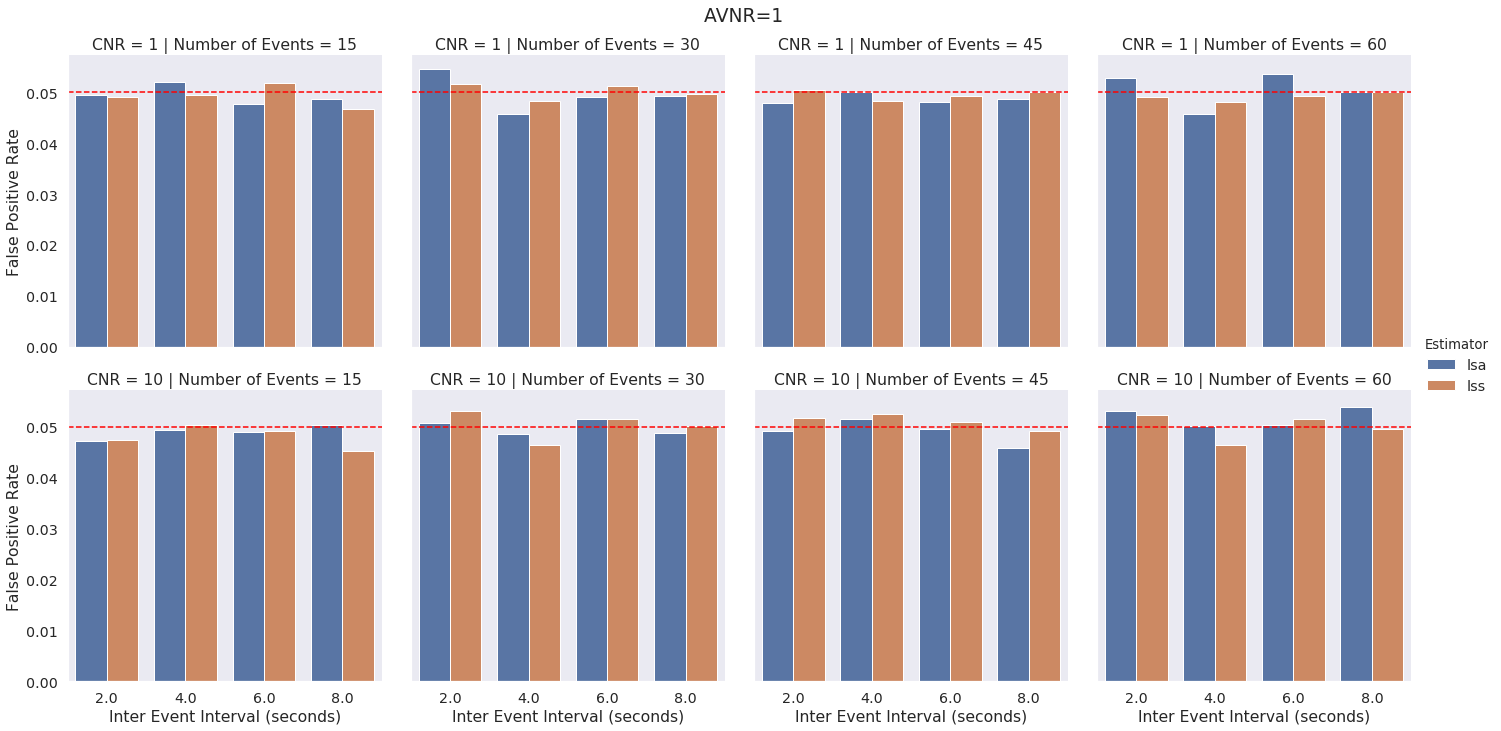
\includegraphics[width=\textwidth]{avnr-1_fpr}}

  \subfloat{\includegraphics[width=\textwidth]{avnr-2_fpr}}

  \caption{
    LSA/LSS both show a \%5 false positive rate for all conditions.
    Each bar represents a sample of 50 pairs of correlations (with no true difference)
    randomly pulled from a distribution of correlations 10,000 times.
  }
  \label{fig:res_sim_fpr}
\end{figure}

With the false positive rate established, we next observed how detectable a
correlation difference of 0.1 was across all parameters.

\begin{figure}[H]
  \centering
  \subfloat{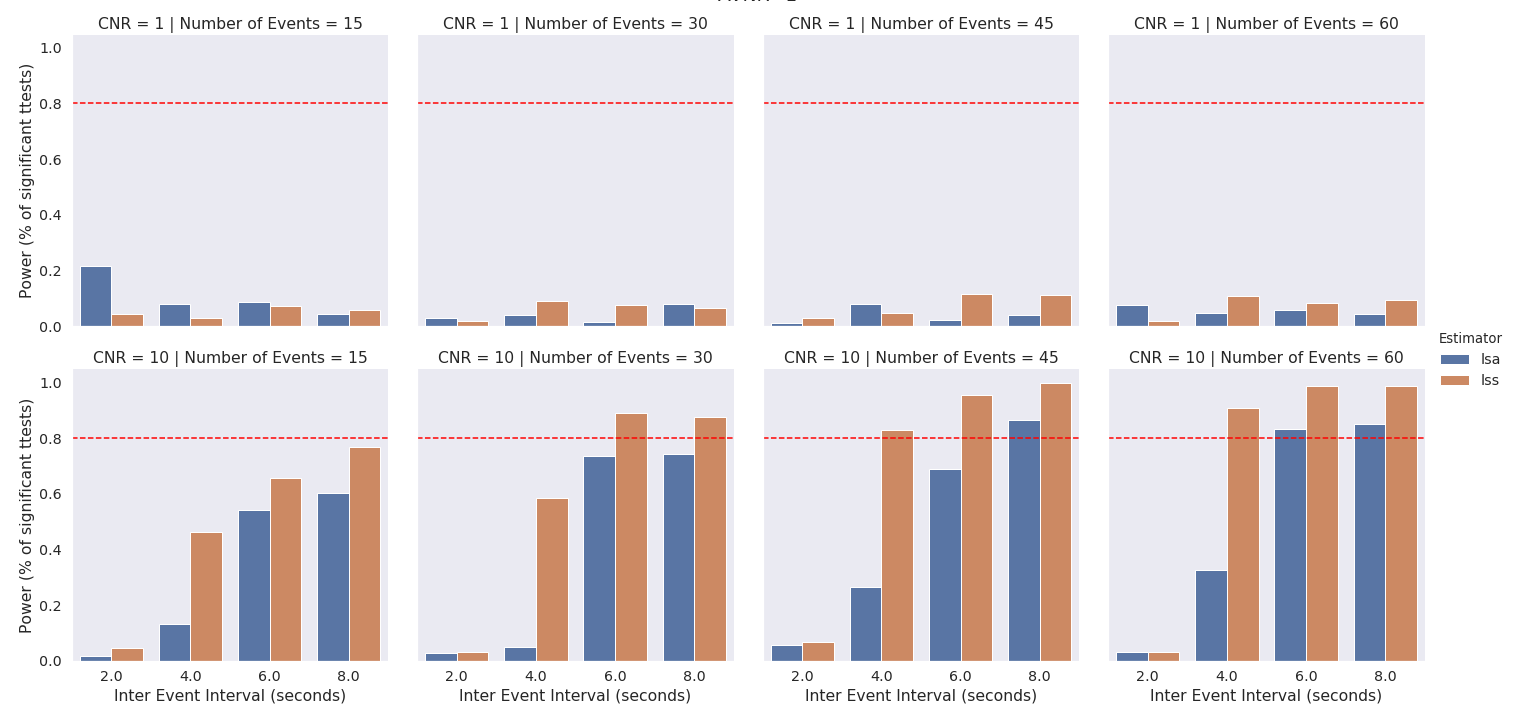
\includegraphics[width=\textwidth]{avnr-1_smalldiff}}

  \subfloat{\includegraphics[width=\textwidth]{avnr-2_smalldiff}}

  \caption{
    Detection power of a small difference between conditions (r=0.1).
    LSS at least marginally outperforms LSA in most simulated experimental
    designs, with a large difference in power when IEI is 4 seconds and
    CNR is high.
    LSS appears to have an advantage in low CNR scenerios across the longer IEIs
    when AVNR is high.
    Each bar represents a sample of 50 pairs of correlations (with no true difference)
    randomly pulled from a distribution of correlations 10,000 times.
  }
  \label{fig:res_sim_smalldiff}
\end{figure}

While the IEI is 2, there is no discernable difference between LSS and LSA.
Since the simulated data were sampled at 2 second intervals, the result
corresponds to effectively presenting a stimulus during each sample.
With such overlapping simulated BOLD responses detecting a difference between conditions
is unlikely.
From an IEI of 4 seconds and upwards, LSS has an advantage over LSA.
Adding additional events above 30 appears to help only if the CNR is greater than 1.
Increasing the CNR improves detection power more than increasing the CVNR, although increasing either
provides a marked boost in detection power.
For LSS, the 8 second IEI does not appear to boost detection power beyond a 6 second IEI,
whereas LSA has a boost when AVNR and CNR are higher.
It's worth noting that even for 50 participants; not one power analysis showed
a power of 80\%, suggesting that larger sample sizes are required to detect a Pearson's R
difference of 0.1.


\subsection*{Task Switching Beta Series Correlations}
\label{results:bsc-taskswitch}

We simulated data using the taskswitching design and found comparable
results to the simulations, with LSS outperforming LSA.
We looked at task switching data from the most lenient
contrast ($real - null$) to the most conserative contrast ($switch - repeat$)
to assess how well LSS and LSA detect ROI-ROI correlation differences between conditions.
For the contrasts $switch - single$, $repeat - single$, and $switch - repeat$ we also
performed the same contrast in the null data to measure the specificity of each method.

The activation atlas is visualized using a glass brain to provide the reader a better sense
of the anatomy.

We found both LSS and LSA had a larger number of statistically significant ROI-ROI pairs
for the contrasts $task - null$ (LSS: 12.86\%; p < 0.001, LSA: 10.48\%; p = 0.001)
and $repeat - switch$ (LSS: 7.62\%; p = 0.047, LSA: 10.00\%; p = 0.005) \ref{fig:main-result}.
Those two contrasts indicate the success of LSS and LSA to measure
condition specific difference in ROI-ROI correlations.
The schaefer atlas has qualitatively similar results (PLACEHOLDER).


\begin{figure}[H]
  \includegraphics[width=\textwidth]{data-real_atlas-activation_participants-filtered_permutation_summary}
  \caption{
    Percentage of statistically significant ROI-ROI pairs observed in the activation atlas
    plotted against a null distribution for the contrasts $task - null$, $switch - single$,
    $repeat - single$, and $switch - repeat$.
    The large dots represent the observed percentage of statistically significant ROI-ROI pairs.
    The violin plots represent 1000 permutations of the data reflecting the null distribution
    of observing statistically significant ROI-ROI pairs.
    The red dashed line represents the expected 5\% false positive rate.
  }
  \label{fig:main-result}
\end{figure}

Although both LSS and LSA detected condition specific correlation differences;
the significant ROI-ROI pairs found with LSS are largely non-overlapping with LSA.

\begin{figure}[H]
  \centering
  \subfloat{\includegraphics[width=\textwidth]{data-both_type-brain_atlas-activation_contrast-taskXnull}}

  \subfloat{\includegraphics[width=\textwidth]{data-task_type-brain_atlas-activation_contrast-repeatXsingle}}

  \caption{
   The statistically significant contrasts $task - null$ and $repeat - single$
   in the real data.
   The glass brains show the anatomical locations of each ROI,
   labelled with its identifying number.
   The edges between ROIs represent significant correlation differences
   between conditions for LSA (blue), LSS (green), or both (yellow).
   The contrast $task - null$ has 22 statistically significant ROI-ROI
   pairs for LSA, 27 statistically significant ROI-ROI pairs
   for LSS with 9 overlapping ROI-ROI pairs for both LSS and LSA.
   The contrast $repeat - single$ has 21 statistically significant ROI-ROI
   pairs for LSA, 16 statistically significant ROI-ROI pairs
   for LSS with 3 overlapping ROI-ROI pairs for both LSS and LSA. 
  }
  \label{fig:significant-contrasts}
\end{figure}

% \begin{table}[!ht]
% \begin{adjustwidth}{-2.25in}{0in} % Comment out/remove adjustwidth environment if table fits in text column.
% \centering
% \caption{
% {\bf Table caption Nulla mi mi, venenatis sed ipsum varius, volutpat euismod diam.}}
% \begin{tabular}{|l+l|l|l|l|l|l|l|}
% \hline
% \multicolumn{4}{|l|}{\bf Heading1} & \multicolumn{4}{|l|}{\bf Heading2}\\ \thickhline
% $cell1 row1$ & cell2 row 1 & cell3 row 1 & cell4 row 1 & cell5 row 1 & cell6 row 1 & cell7 row 1 & cell8 row 1\\ \hline
% $cell1 row2$ & cell2 row 2 & cell3 row 2 & cell4 row 2 & cell5 row 2 & cell6 row 2 & cell7 row 2 & cell8 row 2\\ \hline
% $cell1 row3$ & cell2 row 3 & cell3 row 3 & cell4 row 3 & cell5 row 3 & cell6 row 3 & cell7 row 3 & cell8 row 3\\ \hline
% \end{tabular}
% \begin{flushleft} Table notes Phasellus venenatis, tortor nec vestibulum mattis, massa tortor interdum felis, nec pellentesque metus tortor nec nisl. Ut ornare mauris tellus, vel dapibus arcu suscipit sed.
% \end{flushleft}
% \label{table1}
% \end{adjustwidth}
% \end{table}


%PLOS does not support heading levels beyond the 3rd (no 4th level headings).
% \subsection*{\lorem\ and \ipsum\ nunc blandit a tortor}
% \subsubsection*{3rd level heading} 
% Maecenas convallis mauris sit amet sem ultrices gravida. Etiam eget sapien nibh. Sed ac ipsum eget enim egestas ullamcorper nec euismod ligula. Curabitur fringilla pulvinar lectus consectetur pellentesque. Quisque augue sem, tincidunt sit amet feugiat eget, ullamcorper sed velit. Sed non aliquet felis. Lorem ipsum dolor sit amet, consectetur adipiscing elit. Mauris commodo justo ac dui pretium imperdiet. Sed suscipit iaculis mi at feugiat. 

% \begin{enumerate}
% 	\item{react}
% 	\item{diffuse free particles}
% 	\item{increment time by dt and go to 1}
% \end{enumerate}


% \subsection*{Sed ac quam id nisi malesuada congue}

% Nulla mi mi, venenatis sed ipsum varius, volutpat euismod diam. Proin rutrum vel massa non gravida. Quisque tempor sem et dignissim rutrum. Lorem ipsum dolor sit amet, consectetur adipiscing elit. Morbi at justo vitae nulla elementum commodo eu id massa. In vitae diam ac augue semper tincidunt eu ut eros. Fusce fringilla erat porttitor lectus cursus, vel sagittis arcu lobortis. Aliquam in enim semper, aliquam massa id, cursus neque. Praesent faucibus semper libero.

% \begin{itemize}
% 	\item First bulleted item.
% 	\item Second bulleted item.
% 	\item Third bulleted item.
% \end{itemize}

\section*{Discussion}
\label{discussion}

We provided the first in depth comparison between LSS and LSA to detect condition differences.
We compared LSA and LSS through realistic simulations and a real dataset.
While the simulations suggested LSS is a more powerful measure,
the results from the real dataset do not show a clear winner.
We detail the conclusions from the simulations and the real data, and provide
suggestions for future avenues of research.

% Nulla mi mi, venenatis sed ipsum varius, Table~\ref{table1} volutpat euismod diam. Proin rutrum vel massa non gravida. Quisque tempor sem et dignissim rutrum. Lorem ipsum dolor sit amet, consectetur adipiscing elit. Morbi at justo vitae nulla elementum commodo eu id massa. In vitae diam ac augue semper tincidunt eu ut eros. Fusce fringilla erat porttitor lectus cursus, vel sagittis arcu lobortis. Aliquam in enim semper, aliquam massa id, cursus neque. Praesent faucibus semper libero~\cite{bib3}.
\subsection*{Simulation Conclusions}
\label{discussion:simulation-conclusions}

The main finding from the simulations is that LSS has greater detection power than LSA,
supporting other findings from the literature comparing LSS and LSA using related methods such as
multivariate pattern analysis, representational similarity analysis, and precision of correlations~\cite{Mumford2012,Mumford2014a,Abdulrahman2016,Turner2012a}.
While we cannot control AVNR and CNR in our experiments, we can control the experimental design.
Thus we can offer several suggestions for designing your next experiment based on our simulations.
1) Increasing the IEI up to six seconds improves detection power between conditions substantially,
but increasing the IEI above six seconds only offers modest improvement in detection power.
2) Increasing the number of events per condition to 30 offers the largest benefit in detection power.
It is important to note these recommendations are based on optimized designs made with neurodesign,
and may not generalize to completely random designs.

Abdulrahman \& Henson's (2016) work has also measured various IEIs and varied AVNR and noise coherency between voxels
revealing several key intersections with the present paper.
Increasing the IEI beyond 6 seconds does not appear to help their measure, precision of sample correlation.
Precision of sample correlation measures how accurate the estimated correlation is to the true
simulated correlation.
If the error of the observed correlation is evenly distributed around the
true correlation, then precision of sample correlations would closely mirror our measure of observing
a significant correlation difference between event conditions.
However, if there was a systematic bias in the observed correlations, then precision of sample correlation
would be low, but the correlation difference between event conditions could still be high.
For example, if the true correlations were 0.2 for condition $A$ and 0.3 for condition $B$, but
the observed correlations were 0.1 and 0.2, respectively, then precision of sample correlations would
decrease, but the difference between conditions remains the same.

Another conclusion from Abdulrahman \& Henson's (2016)\cite{Abdulrahman2016} paper suggested to
use LSA when event variability is greater than scan noise (AVNR $>$ 1) for short IEIs (2-5 seconds).
All of our simulations had AVNR greater than or equal to scan noise (AVNR $>=$ 1) and we saw
LSS significantly outperformed LSA for our measure of detection power for IEIs greater than 2 seconds.
Theoretically when AVNR is 1, LSS and LSA would perform similarly, but in our simulations,
LSS still had more power to detect a difference between conditions.
The difference in conclusions could be due to our different measures (i.e., precision of sample correlations versus condition difference)
or from our simulation methods (i.e., guassian noise with random designs versus autocorrelated noise with optimized designs).

Signal and noise coherency did not impact results as they did in the work of Abdulrahman \& Henson (2016)\cite{Abdulrahman2016}.
When scan noise is more coherent across voxels than event variability,
their work states LSA should perform better than LSS.
However, their paper only investigated perfect coherency or no coherency.
In the present simulations, beta series "coherence" was varied between 0.0 and 0.9 Pearson's R correlation,
and the scan noise coherency remained around 0.67 Pearson's R correlation.
For the majority of our simulations, scan noise coherency was greater than beta series
coherence, yet LSS was better at detecting differences between conditions.
It may be the case scan noise must be identical or near identical between voxels
for LSA to perform better than LSS.

The current simulations have improved on previous work by incorporating a more
realistic noise structure using fmrisim and used CNR/AVNR values calculated with real data.
However, the simulations we performed differ from real data in several key areas: the contrasts between event conditions,
variation in BOLD response onset, and preprocessing of the signal.
As mentioned in \nameref{methods:bsc-simulations}, each simulation represents
either a different participant or separate runs from the same participant.
The $real$ and $null$ conditions come from the taskswitching task and resting state,
respectively, representing two runs.
The contrasts in the simulations are therefore most analogous to the $real - null$
contrast in \ref{fig:significant-contrasts}.
Additionally, each simulation contains two conditions whose BOLD responses
are independent of each other, that is, the BOLD response for one event
does not influence the BOLD response for a subsequent event.
There is likely temporal autocorrelation of BOLD responses across events,
which is not represented in our simulations ~\cite{Abdulrahman2016}.

We also did not simulate variations in BOLD response onset, which is likely to occur
as all BOLD responses to a stimulus do not occur at the time the stimulus onset ~\cite{DEsposito2003}.
Model mismatch through variations has been found detrimental to beta estimation, 
but there is no reason to believe that LSA would be differentially impacted relative to LSS ~\cite{Turner2012a}.
Future work could investigate variable BOLD responses and include derivatives for each regressor to account for
the variable BOLD responses.
Including derivatives could make LSA unsolvable since every event would have at least two regressors, meaning
there must be more than twice the volumes than events collected during the BOLD run
for the GLM to be solvable.

While the simulations represented data without any preprocessing applied,
the real data had several variables included in the model: motion outliers, non-steady state volumes,
CSF, and white matter signals.
The additional regressors in the model reduce the degrees of freedom
and could impact the ability of the model to fit the data.
This would likely impact LSA more than LSS, since LSA already contains
a large number of regressors representing each event.
Future work could use fmrisim to simulate entire brains and preprocess them with fmriprep,
which would make the processing pipeline between simulated and real data closer.

\subsection*{Real Data Conclusions}
\label{discussion:taskswitching-conclusions}

The real data suggests LSS and LSA perform similarly.
Based on the number of statistically significantly different ROI-ROI pair correlations alone,
LSS and LSA cannot be easily distinguished.
Overall, we have evidence LSA and LSS are able to detect differences between
blocks of events ($task - null$ and $repeat - single$), but not within blocks of events ($switch - repeat$).
The latter contrast would be a common contrast seen in fast event-related designs suggesting
great care should be taken to determine if you have enough power to detect differences
between conditions.

Contrary to the simulations where LSS was found to be more powerful,
there is some evidence of LSS having fewer statistically significant ROI-ROI pairs than expected through chance alone
for the contrast $switch - repeat$.
This result either suggests there are not many ROI-ROI pairs that do change their correlation
between the two conditions, or that LSS has poor sensitivity to detect those differences.
Since there is not a strong theoretical backing to say the pattern of results
in LSS is closer to the ground truth than LSA, we cannot say which
explanation above is more likely.

A surprising result is the lack of overlap between LSS and LSA significant ROI-ROI pair correlation differences.
The lack of overlap is suprising because both LSS and LSA are purported to
measure the same underlying process of task related connectivity.
We correlated the beta series from LSA to LSS and plotted that relationship with
average framewise displacement and temporal signal to noise (TSNR) for all participants ($N$=61) to investigate this surprising result. \ref{fig:lss_lsa_correlation}.
As the average framewise displacement increases and temporal signal to noise (TSNR)
decreases, the agreement between LSS and LSA decreases.
In other words, as noise in the data increases, the more divergent LSS and LSA become.
This suggests one reason for the disagreement is the noise present in the included
data.
There appears to be a cluster of particpants with an average framewise displacement of
less than 0.2mm that have a high correlation between LSS and LSA.
The simulation results would suggest when LSS and LSA disagree, the estimate for LSS should be
trusted, but since we observed a significant number of condition modulated ROI-ROI pair correlations for both
LSS and LSA, it is difficult to say whether LSA or LSS would be "correct".

\begin{figure}[H]
  \centering
  \includegraphics{lss_lsa_noise_relationship}
  \caption{
    The average correlation between LSA/LSS beta series across
    all ROIs in the activation atlas.
    Orange dots represent 21 participants that were not included
    in the original analysis and blue dots are the 40
    participants that were included.
    The size of the dots represent the temporal signal to noise
    ratio (TSNR), higher is better.
    The general pattern shows good correspondence between LSA and LSS
    when the average framewise displacement is low and TSNR is high.
  }
  \label{fig:lss_lsa_correlation}
\end{figure}

Another interesting aspect of our analysis of the real data was the inclusion of
null (resting state) data where the participants simply stared at a fixation cross.
It could be argued the resting state data does not provide an adequate null model
to compare to the real task data because there is presumably no BOLD response at any
of the onset times.
Trying to model the BOLD response with no expectation of a BOLD response existing could lead
to large misfits and deviating beta estimates.
To test this, we evaluated average CNR and AVNR within the Schaefer and activation atlases in
the null data and compared it to the CNR and AVNR in the real data.
If the null data had much larger deviations in beta estimates, CNR and AVNR would be higher
in the null data relative to the real data.
For both LSS and LSA, the Schaefer atlas had statistically significantly higher
CNR/CVNR in the null data relative to the real data, whereas the activation atlas
did not show a statistically significant difference between null and real data \ref{table2}.

\begin{table}[H]
  \begin{adjustwidth}{0in}{0in} % Comment out/remove adjustwidth environment if table fits in text column.
  \centering
  \caption{
  {\bf Differences in CNR/AVNR between real and null data}}
  \begin{tabular}{|l+l+l|l|l|l|}
  \hline
  Atlas & Method & CNR (t-value) & CNR (p-value) & AVNR (t-value) & AVNR (p-value)\\ \thickhline
  $Schaefer$ & $LSS$ & 3.163 & \textbf{0.003} & 3.659 & \textbf{0.001}\\ \hline
  $Activation$ & $LSS$ & 0.105 & 0.917 & 1.528 & 0.134\\ \hline
  $Schaefer$ & $LSA$ & 2.740 & \textbf{0.009} & 2.893 & \textbf{0.006}\\ \hline
  $Activation$ & $LSA$ & 0.306 & 0.761 & 0.927 & 0.360\\ \hline
  \end{tabular}
  A t-test comparing average CNR/AVNR across all ROIs between real data and null data.
  A statistically significant p-value ($p < 0.05$) suggests the CNR/AVNR value in the real data
  is different from the null data.
  Only CNR/AVNR from the Schaefer atlas shows statistically significant results.
  \label{table2}
  \end{adjustwidth}
  \end{table}

The table suggests model misfit may be a driving factor for spurious results in the Schaefer atlas.
We protected against extreme beta estimates by detecting and removing outliers, but model misfit
could still drive spurious results.
A proper null model would have bold responses at the onset times, but the bold responses
would be the same amplitude at every event such that the only deviance in the simulated
BOLD responses would come from the underlying resting state fluctuations.

\subsection*{Future Directions}

There are several immediate next steps that could be taken to provide a more concrete answer
on when one should use LSA or LSS when looking at ROI-ROI pair correlation differences between event
conditions.

With the publically available NiBetaSeries package, researchers could replicate the
results on their own data using the same methods in this paper.
Furthermore, there are several analytical choices that could be varied using NiBetaSeries such as:
using a t-statistic instead of a raw beta estimate, including derivatives of the hemodynamic response function,
and performing a spatial-temporal analysis using finite impulse responses.
The benefit of using a t-statistic is the added stability of the estimates.
The t-tstatistic will scale outlier beta estimates with large uncertainty giving more stability
towards the beta series estimates.
Since LSA is more likely to produce high variance beta estimates, using a t-statistic would likely impact
how well LSA performs.
No other tool has the option to calculate the t-statistic instead of the raw beta estimate to the knowlege
of the authors.
Another straight-forward addition would be adding temporal and/or dispersion derivatives to each beta
estimate to account for potential BOLD response delays ~\cite{Calhoun2004,Gottlich2015}.
This strategy may work well for populations with variable BOLD responses or when the onset of the BOLD
response is not precisely known.
Including derivates would also likely impact LSA more than LSS since there would be either twice or
three times the number of regressors included in the LSA model, which in a fast event-related design
would heavily impact the degrees of freedom in the model.
Finally, a more complex but potentially fruitful option is to use the finite impulse response model.
Finite impulse responses allow the researcher to observe both the spatial and temporal pattern of
condition specific correlation without imposing an expected shape of the hemodynamic response ~\cite{Turner2012a}.
For example, the researcher could be able to determine the relationship between two event conditions
two, four, six, and eight seconds post stimulus, and identify how that relationship changes across
that time frame.
The finite impulse response model can only be estimated using LSS, giving LSS the advantage if researchers
want to perform this type of analysis.

Network measures of brain organization are becoming widely adopted ~\cite{Rubinov2010}.
Network measures offer a perspective on the total organization of ROI-ROI pairs, instead of
interrogating individual ROI-ROI pairs as we did in the present work.
Previous work has found greater global efficiency, smaller mean clustering coefficients, and lower modularity in
task relative to rest ~\cite{Di2013}.
However, this finding has not been replicated using beta series correlations and has just begun
to be investigated between tasks and event conditions within a task ~\cite{Di2019a}.
The largely non-overlapping results from LSS and LSA suggest that LSS and LSA may differ
in their network measures as well.
% \begin{itemize}
%   \item Run beta series correlations on larger dataset with enough power to reliably detect an effect
%   \item Add ability to estimate CNR/AVNR in NiBetaSeries
%   \item use t-statistic as opposed to raw beta estimates
%   \item temporal/spatial analysis with Finite Impulse Responses \cite{Turner2012a}
%   \item Add ability to simulate possible condition relationships in NiBetaSeries
%   \item need to add "fake" mean hemodynamic response to normalize the data
%   \item extend Cole's work (compare residual correlations with LSA/LSS)
%   \item investigate graph theoretical measures to validate between task conditions and task/null.
%   \item simulate variable onset of BOLD responses
%   \item use ds00030 to validate results on publically available dataset already analyzed with BSC ~\cite{Di2019a}
% \end{itemize}
% \subsection{Limitations}

% \begin{itemize}
%   \item Mixing of noise parameters may not be representative of real data
%   \item The contrasts in the simulated data do not represent a true mixing of different event types
%   \item Did not have enough participants to measure a robust effect (other studies had fewer participants)
%   \item The preprocessing of the MRI data was minimal, (data could potentially be made less noisy)
% \end{itemize}

\section*{Conclusion}

In conclusion, while our simulations suggested LSS has more power than LSA to
detect differences between conditions, the real data suggests LSA and LSS perform similarly.
LSA may be better suited 
LSS may be worse at detecting differences between conditions when they are interspersed
with each other and not separated by blocks.
The null data also suggest inflated positives when the data are between blocks,
suggesting the differences between blocks are likely partially driven by something other than
task evoked BOLD response variability.


% CO\textsubscript{2} Maecenas convallis mauris sit amet sem ultrices gravida. Etiam eget sapien nibh. Sed ac ipsum eget enim egestas ullamcorper nec euismod ligula. Curabitur fringilla pulvinar lectus consectetur pellentesque. Quisque augue sem, tincidunt sit amet feugiat eget, ullamcorper sed velit. 

% Sed non aliquet felis. Lorem ipsum dolor sit amet, consectetur adipiscing elit. Mauris commodo justo ac dui pretium imperdiet. Sed suscipit iaculis mi at feugiat. Ut neque ipsum, luctus id lacus ut, laoreet scelerisque urna. Phasellus venenatis, tortor nec vestibulum mattis, massa tortor interdum felis, nec pellentesque metus tortor nec nisl. Ut ornare mauris tellus, vel dapibus arcu suscipit sed. Nam condimentum sem eget mollis euismod. Nullam dui urna, gravida venenatis dui et, tincidunt sodales ex. Nunc est dui, sodales sed mauris nec, auctor sagittis leo. Aliquam tincidunt, ex in facilisis elementum, libero lectus luctus est, non vulputate nisl augue at dolor. For more information, see \nameref{S1_Appendix}.

\section*{Supporting information}

% Include only the SI item label in the paragraph heading. Use the \nameref{label} command to cite SI items in the text.
% \paragraph*{S1 Fig.}
% \label{S1_Fig}
% {\bf Bold the title sentence.} Add descriptive text after the title of the item (optional).

% \paragraph*{S2 Fig.}
% \label{S2_Fig}
% {\bf Lorem ipsum.} Maecenas convallis mauris sit amet sem ultrices gravida. Etiam eget sapien nibh. Sed ac ipsum eget enim egestas ullamcorper nec euismod ligula. Curabitur fringilla pulvinar lectus consectetur pellentesque.

% \paragraph*{S1 File.}
% \label{S1_File}
% {\bf Lorem ipsum.}  Maecenas convallis mauris sit amet sem ultrices gravida. Etiam eget sapien nibh. Sed ac ipsum eget enim egestas ullamcorper nec euismod ligula. Curabitur fringilla pulvinar lectus consectetur pellentesque.

% \paragraph*{S1 Video.}
% \label{S1_Video}
% {\bf Lorem ipsum.}  Maecenas convallis mauris sit amet sem ultrices gravida. Etiam eget sapien nibh. Sed ac ipsum eget enim egestas ullamcorper nec euismod ligula. Curabitur fringilla pulvinar lectus consectetur pellentesque.

% \paragraph*{S1 Appendix.}
% \label{S1_Appendix}
% {\bf Lorem ipsum.} Maecenas convallis mauris sit amet sem ultrices gravida. Etiam eget sapien nibh. Sed ac ipsum eget enim egestas ullamcorper nec euismod ligula. Curabitur fringilla pulvinar lectus consectetur pellentesque.

% \paragraph*{S1 Table.}
% \label{S1_Table}
% {\bf Lorem ipsum.} Maecenas convallis mauris sit amet sem ultrices gravida. Etiam eget sapien nibh. Sed ac ipsum eget enim egestas ullamcorper nec euismod ligula. Curabitur fringilla pulvinar lectus consectetur pellentesque.

\section*{Acknowledgments}
This work could not have been completed without the support of several persons/resources.
First, the simulation analyses were supported in part through computational resources provided by The University of Iowa, Iowa City, Iowa.
Second, the design and support of the study providing the real data was given by Hyku Lee, funded by grant INSERT GRANT NUMBER.
Third, Chris Oeler and Adriana-Rivera Dompencial collected the real data used in the data analysis.

\section*{Author Contributions}
JK and MV conceptualized this work, CB and MV funded the study collecting the real data,
JK performed the analyses, and JK wrote the manuscript.

\nolinenumbers

\bibliography{plos}
% Either type in your references using
% \begin{thebibliography}{}
% \bibitem{}
% Text
% \end{thebibliography}
%
% or
%
% Compile your BiBTeX database using our plos2015.bst
% style file and paste the contents of your .bbl file
% here. See http://journals.plos.org/plosone/s/latex for 
% step-by-step instructions.
% 
% \begin{thebibliography}{10}

% \bibitem{bib1}
% Conant GC, Wolfe KH.
% \newblock {{T}urning a hobby into a job: how duplicated genes find new
%   functions}.
% \newblock Nat Rev Genet. 2008 Dec;9(12):938--950.

% \bibitem{bib2}
% Ohno S.
% \newblock Evolution by gene duplication.
% \newblock London: George Alien \& Unwin Ltd. Berlin, Heidelberg and New York:
%   Springer-Verlag.; 1970.

% \bibitem{bib3}
% Magwire MM, Bayer F, Webster CL, Cao C, Jiggins FM.
% \newblock {{S}uccessive increases in the resistance of {D}rosophila to viral
%   infection through a transposon insertion followed by a {D}uplication}.
% \newblock PLoS Genet. 2011 Oct;7(10):e1002337.

% \end{thebibliography}



\end{document}
